\newpage
% ML: anglictina v nazvu casti (plati pro celou praci)

\part{Webové publikační mapové platformy}
\newpage
\section{Principy platforem}
%\label{sec:WPS}

%moznost pridani ilustrativniho obrazku
\subsection{Mapy a internet}

Lidé vytvářejí mapy odjakživa, ale již dávno je dobám kdy bylo nutné
pro nahlédnutí mapy mít její fyzický otisk či originál. Problémem
takových map je jejich nákladná distribuce a omezené možnosti
obsahu. Mnohem efektivnější způsobem jak distribuovat mapy pro
veřejnost se v dnešní době stávají webové mapové platformy. Možná
nejslavnější z nich \textit{Google Maps} byla spuštěná již začátkem
roku 2005 \cite{google_history}.  Obecně se mapové platformy dělí na
dvě skupiny: statické a interaktivní.

\textbf{Statické mapové platformy} nejsou z důvodu jejich úzkého
zaměření dnes již tolik běžné, avšak tvorba jejich obsahu je oproti
mapám interaktivním velice snadná. Publikované mapy se dají vytvořit
přímo pomoci specializovaných kartografických programů, nebo scanem
již existujících map. Takto vytvořené podklady jsou na webu velice
snadno distribuovatelné a kladou výrazně menší nároky na výpočetní
techniku.

Jak již název napovídá \textbf{interaktivní mapové platformy} jsou
takové platformy, u kterých má možnost uživatel měnit jejich
obsah. Nejčastěji se jedná o výběr podkladové mapy, filtraci mapových
prvků, přibližování a oddalování. Zjednodušeně řečeno se jedná o
interakci uživatele s webovým rozhraním dané aplikace, která dle
uživatelem kladených příkazů opakovaně aktualizuje svůj
obsah\cite{web_mapping}. Tato zkutečnost dělá z interaktivních map
velice účinný nástroj. Na druhou stranu je nutné říci, že výroba a
distribuce map pro takové platformy je o poznání složitější.

\newpage
\subsection{Fungování interaktivních mapových platforem}

V dnešní době se hlavně v očích uživatelů těší většímu zájmu právě
interaktivní mapové platformy. Proto se jimi tato podkapitola bude
zajímat více podrobně.

Existuje velké množství interaktivních mapových platforem, jejich
základní princip fungování je však ve většině případů stejný a liší se
pouze svými možnostmi, obsahem a využitím.

\begin{figure}[h!]
	\centering
	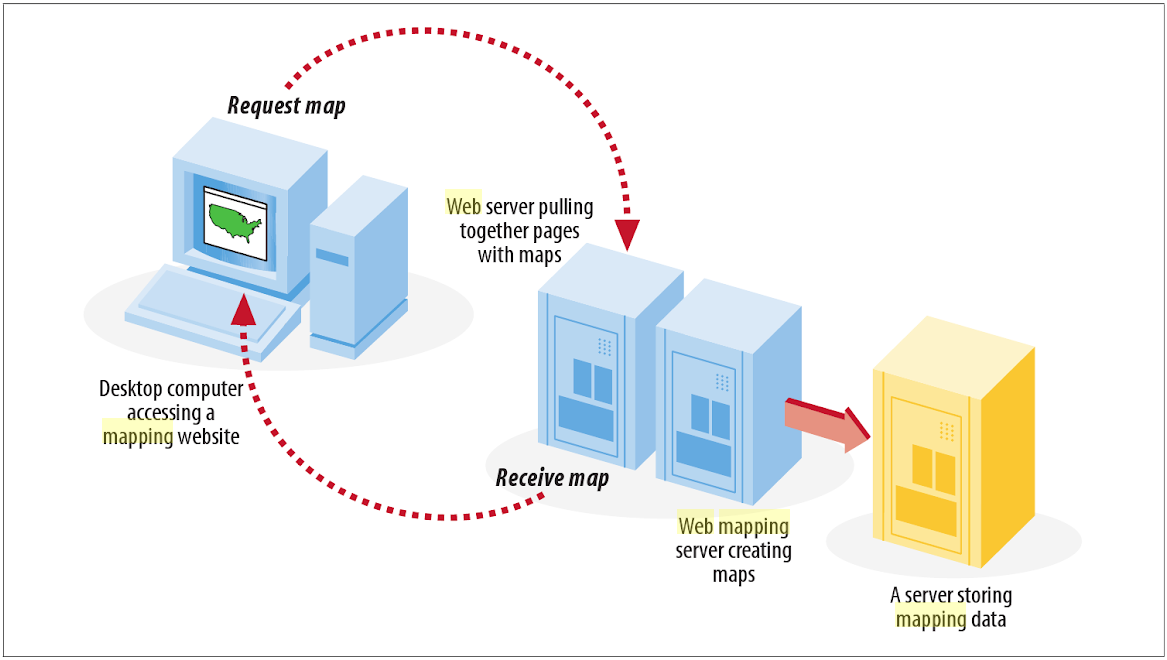
\includegraphics[width=1\textwidth]{../img/map-web-diagram.png}
	\caption{diagram znázorňující interakci uživatele a částí webové aplikace uložené na servrech: \cite{web_mapping}}
	\label{fig:WPS_class_diagram}
\end{figure}

V obrázku 1 je znázorněn jednoduchý diagram, který popisuje fungování
interaktivní webové aplikace a jejích základních komponentů. Při
pohledu zleva se jedná především o tyto části:

\textit{Koncové zařízení} označované také jako webový klient,
využívající počítač, tablet, nebo mobilní telefon. Výsledná rychlost a
požitek z webové aplikace dnes již není limitován tolik výpočetní
rychlosti klienta, spíš jako rychlostí internetového
připojení. Všechnu nutnou komunikaci přitom zastává webový prohlížeč,
který je pomocí \textit{request URL} získává informace z hostujícího
serveru, na kterém je webová aplikace reálně uložena.

\textit{Webový server} přijímá požadavky od klienta a zastává nutnou
komunikaci mezi mapovým serverem a uložištěm dat. Na webovém serveru
je uložena aplikace a na vyžádání poskytuje obsah webové aplikace
klientovy.

\textit{Webový mapový server} jedná se o program, který na základně
požadavků poslaných od webového serveru a dat z uložiště vytvoří
požadovaný mapový obraz a odešle jej zpět. Mapových serverů existuje
více. Těm nejvíce používaným se bude věnováno v dalších kapitolách.

\textit{Uložiště dat} zde jsou fyzicky uložena všechna data potřebná k
vytvoření mapy, nebo její části. Jedná se o rastrová, či vektorová
mapová data ve vhodném formátu, který dokáže webový mapový server
zpracovat. Dále jsou zde uložena metadata, která jsou nutnou součástí
prostorových dat. Popisují data sloužící k vytvoření mapy a dále
jejich původ, způsob použití a samotný obsah dat \cite{web_mapping}.

Důležitou součástí každé webové mapové aplikace je samotná komunikace
mezi jednotlivými jejími komponenty. V následujících podkapitolách
bude brán zřetel převážně na komunikaci mezi webovým klientem a
webovým mapovým serverem. Konkrétně na protokoly, které jsou používané
pro získání mapového obrazu. Tyto standarty jsou poskytovány
mezinárodní standardizační organizací \textit{Open Geospatial
  Consortium (OGC)}

\subsection{Open Geospatial Consortium}

Open Geospatial Consortium (OGC) je mezinárodní nezisková organizace
zahrnující komerční, vědecké, vládní a nevýdělečné organizace, které
se zabývají vytvářením kvalitních specifikací pro prostorová
data. Tyto specifikace jsou jsou volně dostupné pro kohokoli za účelem
zlepšení sdílení prostorových dat po celém světě \cite{oqc_web}.

OGC specifikace jsou technické dokumenty detailně popisující rozhraní,
nebo kódování. Tyto dokumenty jsou dále použity na straně vývojářů ke
tvorbě jejich produktů. Hlavní myšlenka je taková, že dva nezávisle
vyvíjené programy používající OGC standarty by měly být vzájemně
kompatibilní \cite{oqc_web}. Celkem se jedná o více než 50
specifikací, více konkrétně se však budou popsány pouze následující:

\newpage
\begin{itemize}
\item\textit{Web Map Services (WMS)} - WMS nabízí jednoduché HTTP
  rozhraní pro posílání žádostí o georeferencovaný mapový obraz. Na
  základě WMS dotazu server odpoví odesláním rastrové mapy, která
  obsahuje požadované mapové prvky v daném výřezu (dlaždice).
	 
\item\textit{Web Map Tile Services (WTMS)} - princip fungování WMTS
  komunikace klient-server obdobný jako u WMS. Hlavní rozdíl je však v
  tom, že požadované dlaždice jsou již předem vytvořeny a uloženy
  interní paměti serveru. Server je tedy nemusí při každém dotazu
  znovu vytvářet, což při jeho velkém množství dotazů celý proces
  výrazně zrychlí.
\end{itemize}

\subsection{Web Map Services (WMS)}

WMS, v českém překladu webový mapový servis, na základě geografických
informací vytváří georeferencované mapy. Mezinárodní standart dále
definuje "mapu" jako digitální vyobrazení geografických informací,
které je vhodné pro počítačové obrazovky a displeje. V případě mapy
jako takové se tedy nejedná o data, ale o jejich produkt. Mapy
vytvořené na základě WMS specifikace mohou být v obecných formátech
např. PNG, GIF, nebo JPEG. Méně často se také jedná o vektorovou
grafiku ve formátech SVG, nebo WebCGM \cite{oqc_wms}.

Popisovaný standart definuje několik operací, každou s odlišným
výstupem. Tyto operace vrací dávají uživateli buďto informace o
samotném servisu, poskytují mapu, nebo informace o zobrazovaných
mapových prvcích.

\begin{itemize}

\item\textit{GetCapabilities} - operace vrací dokument ve formátu XML,
  který obsahuje veškeré informace nutné k vytvoření \textit{GetMap}
  požadavku. Jedná se tedy o detaily samotného servisu jako
  takového. Pomocí GetCapabilities lze zjistit počet vrstev, jejich
  souřadnice v referenčním systému atd.
	
\item\textit{GetMap} - jedná se o nejdůležitější operaci, protože
  jejím výsledkem je samotný geolokalizovaný mapový obraz. K jeho
  získání je potřeba poskytnout sadu parametrů, na základě kterých je
  v mapovém serveru vytvořen. Těmto parametrům bude věnována další
  podkapitola.
	
\item\textit{GetFeatureInfo} - operace vrací informace o prvcích
  zobrazených na mapě.
	
\item\textit{GetLegendGraphic} - dle poskytnutých parametrů vytvoří
  tato operace legendu, kterou server vrátí jako obraz ve zvoleném
  formátu.
\end{itemize}

\subsection{Parametry WMS}

Parametry obecně slouží ke specifikaci úkonu, který od mapového
serveru požadujeme. Jedná se tedy o vstupní informace na základě
kterých nám server odpoví. Parametrů je velké množství, některé jsou
používány vždy, některé jen velice ojediněle. Možnosti použití
parametrů se liší dle operace (requestu), kterou provádíme.

Níže uvedené parametry se vztahují pouze k operaci
\textbf{\textit{GetMap}}. U operací jako \textit{GetCapabilities},
nebo \textit{GetFeatureInfo} může bý popsaný význam parametrů odlišný,
nebo není možné parametr použít vůbec.

\begin{itemize}
\item\textit{VERSION} - specifikace verze WMS.
	
\item\textit{REQUEST} - výběr provedené operace (v případě požadavku o
  mapu se jako request parametr použije "GetMap".
	
\item\textit{LAYERS} - list oddělený čárkami obsahující názvy vrstev,
  které budou použity pro tvorbu mapy
	
\item\textit{STYLES} - list oddělený čárkami, který definuje jakým
  stylem se budou jednotlivé vrstvy vykreslovat. List stylů proto musí
  korespondovat s listem vrstev. Pro implicitní hodnoty je možné
  použít "STYLES=".
	
\item\textit{SRS} - zkratka SRS v překladu znamená "geodetický
  referenční systém". Tímto parametrem je tedy určeno v jakém
  geodetickém referenčním systému jsou poskytnuté parametry
  např. BBOX. Rovněž se jedná o určení referenčního systému pro
  výsledný mapový obraz.
	
\item\textit{BBOX} - jedná se o souřadnice výřezu pro který generuje
  výsledný mapový obraz. Pro definování výřezu je třeba zadat
  souřadnice levého spodního a pravého horního rohu. Pole souřadnic
  tedy parametr vypadá následovně "minX,minY,maxX,maxY".
	
\item\textit{FORMAT} - nastavení formátu výstupního souboru (mapového
  obrazu). Nejčastěji používané jsou formáty GIF, PNG, JPEG, které
  mohou být jednoduše zobrazeny na webových prohlížečích. Je však
  možnost nastavit formát také jako SVG, nebo WebCMG.
	
\item\textit{WIDTH} - celočíselná hodnota udávající šířku výsledné
  mapy v pixelech. Jinak řečeno se jedná o vzdálenost v pixelech mezi
  body zadané parametrem \textit{BBOX} tj. vzdálenost minx a maxx.
	
\item\textit{HEIGHT} - hodnota odpovídající parametru \textit{WIDTH} s
  tím rozdílem, že se jedná o vzdálenost miny a maxy. Pokud je poměr
  stran \textit{WIDTH}/\textit{HEIGHT} odlišný od poměru stran
  \textit{BBOX} je výsledný rozměr v pixelech přizpůsoben poměru stran
  \textit{BBOX}.
	
\item\textit{TRANSPARENT} - udává zda-li je mapové pozadí průhledné,
  nebo ne.
\end{itemize}

Mezi další méně používané parametry patří např. \textit{EXCEPTIONS},
\textit{TIME}, \textit{ELEVATION}, \textit{BGCOLOR} \cite{oqc_wms}.

Výše uvedené parametry lze rozdělit na dvě části a to povinné a
nepovinné viz. tabulka:

\bigskip
\begin{table}[h!]
	\catcode`\-=12
	\centering
	\begin{tabular}{|c|c|}
		\hline
		parametr & povinný \\ \hline
		\hline
		VERSION & ano \\ \hline
		REQUEST & ano \\ \hline
		STYLES & ano \\ \hline
		SRS & ano \\ \hline
		BBOX & ano \\ \hline
		WIDTH & ano \\ \hline
		HEIGHT & ano \\ \hline
		TRANSPARENT & ne \\ \hline
		EXCEPTIONS & ne \\ \hline
		TIME & ne \\ \hline
		ELEVATION & ne \\ \hline
		BGCOLOR & ne \\ \hline
\end{tabular}
	\caption{Výpis parametrů a jejich povinnost použití: \cite{oqc_wms}}
	\label{tab:WPS_ExecuteRequest}
\end{table}

\subsection{Parametr TIME}

S ohledem na téma této práce je vhodné přiblížit si parametr
\textit{TIME} více podrobně a popsat způsob jeho použití a možnosti,
které nabízí.

Dle OGC je formát parametru \textit{TIME} dán normou ISO 8601:1988(E),
která rozšiřuje normu ISO 8601. Oproti té jsou přidány další
specifikace\cite{oqc_wms}:
%http://cite.opengeospatial.org/OGCTestData/wms/1.1.1/spec/wms1.1.1.html#basic_elements.params.time
\begin{itemize}
\item Syntax pro datové kolekce. Jejich začátek, konec a periodické
  opakování.
\item Definice speciálních znaků pro vyjádření sedmi dní v týdnu.
\item Možnost zadání data před rokem 1 našeho letopočtu a to až do
  časově vzdálených geologických období (milióny a miliardy let v
  minulosti).
\end{itemize}

Základní časový formát ISO 8601:1988(E) rozšířené normy umožňuje
specifikovat časový formát až na úroveň tisícin sekund. Né pro každou
hodnotu je však vyžadována takováto přesnost. Proto lze formát upravit
tak, že jsou odstraněny zpřesňující číslice.

\noindent
Základní formát vypadá následovně:

\begin{verbatim}
ccyy-MM-ddThh:mm:ss.SSSZ
\end{verbatim}

\noindent
A jeho zjednodušená forma pro vyjádření hodnoty s přesností na dny:

\begin{verbatim}
ccyy-MM-dd
\end{verbatim}

\newpage
\noindent
V ukázkách časových formátů jsou použita jednotlivá označení:

\begin{itemize}
	\item cc \textit{2 číslice století}
	\item yy \textit{2 číslice rok}
	\item MM \textit{2 číslice měsíc}
	\item dd \textit{2 číslice den}
	\item hh \textit{2 číslice hodina}
	\item mm \textit{2 číslice minuta}
	\item ss \textit{2 číslice sekunda}
	\item SSS \textit{3 číslice milisekunda}
\end{itemize}

\begin{itemize}
	\item T \textit{slouží k oddělení hodnot určující den a hodnot určující čas uvnitř dne}
	\item Z \textit{slouží k definici časového pásma vztaženému ke koordinovanému světovému času UTC}
\end{itemize}

Speciální znaky pro zadávání dnů v týdnu jsou: 'MON', 'TUE', 'WED',
'THU', 'FRI', 'SAT', 'SUN'. Pravěká období se definují např: M150
\textit{150 mil. let před Kristem (období Jura)}, K18 \textit{pozdní
  Doba ledová}

\newpage
\section{Webové mapové platformy}

Mapových publikačních platforem existuje v dnešní době velké
množství. Mohou být přizpůsobeny účelu za kterým jsou vytvořeny, nebo
konkrétním vstupním datům s kterými pracují. Né tedy všechny mají
integrovanou podporu pro práci s časoprostorovými daty. Tato
skutečnost je zároveň způsobena tím, že časoprostorová data nejsou
podporována všemi mapovými servery. Právě podpora na straně webového
mapového serveru je při tvorbě mapové publikační platformy
klíčová. Jak se ale dozvíme dál v práci, né nutná.
 
Tato kapitola se zabývá jednotlivými webovými mapovými servery a
jejich možnostem podpory časoprostorových dat. Jednotlivé podkapitoly
jsou vždy věnovány jednomu webovému mapovému serveru, který bude
představen a dále bude popsán způsob podpory časoprostorových dat. U
některých mapových serverů je závěr každé podkapitoly je přidaná
ukázka z webových mapových platforem využívající konkrétní mapový
server.

\subsection{MapServer}

\begin{figure}[h!]
	\centering
	
\includegraphics[width=0.4\textwidth]{../img/mapserver-logo.png}
	\label{fig:mapserver-logo}
\end{figure}
\bigskip

MapServer je platforma s otevřeným kódem, která byla vytvořena pro
publikaci prostorových dat a interaktivních mapových aplikací. Byla
vytvořena devadesátých letech v Minnesotské univerzitě. V té době se
jednalo o jeden z prvních podporovaných projeků organizací OSGeo. Je
nutno podotknout, že MapServer není a ani nebyl navržen jako
stoprocentní GIS systém. Důvod jeho vzniku je dán potřebou organizací
NASA, která hledala způsob jakým zprostředkovat satelitní snímky
veřejnosti. MapServer je psaný v jazyce C a podporuje všechny hlavní
operační systémy jakou jsou Windows, Linux a Mac OS X
\cite{mapserver_about}.

\bigskip
\noindent
\textbf{Podpora časových dat}

Od verze 4.4 je v MapServeru přidána podpora, která dokáže
interpretovat WMS parametr TIME obsahující časovou hodnotu. MapServer
tuto hodnotu zpracuje a v requestu vrátí odpovídající mapový obraz.

K tomu, aby bylo možné jednotlivé vrstvy selektovat pomocí atributu
TIME, musí každá vrstva obsahovat následující metadata
\cite{mapserver_about}:

\begin{itemize}
\item\textit{wms-timeextent} - povinná hodnota obsahující interval
  časových hodnot, které vrstva obsahuje. Tento interval lze zjistit
  pomocí operace. \textit{GetCapabilities}.
\item\textit{wms-timeitem} - povinná hodnota obsahující název záznamu
  v databázi, ve kterém jsou časová data uložena.
\item\textit{wms-timedefault} - nepovinná hodnota určující implicitní
  hodnotu v případě, že časová hodnota pro daný záznam chybí.
\end{itemize}

\noindent
Záznam obsahující vrstvu s časoprostorovými daty vypadá následovně:

\begin{verbatim}
LAYER
	NAME "earthquakes"
	METADATA
	"wms_title"    "Earthquakes"
	"wms_timeextent" "2004-01-01/2004-02-01"
	"wms_timeitem" "TIME"
	"wms_timedefault" "2004-01-01 14:10:00"
	"wms_enable_request" "*"
	END
	TYPE POINT
	STATUS ON
	DATA "quakes"
	FILTER (`[TIME]`=`2004-01-01 14:10:00`)
	CLASS
	..
	END
END
\end{verbatim}

\bigskip
\noindent
\textbf{Formáty časových dat a syntaxe}

% moznost pridat tabulku podporovanych formatu
Výhodou použití MapServeru je jeho podpora dalších časových formátů,
které nejsou v normě ISO 8601:1988(E) používané pro operaci
\textit{WMS TIME} definovány. Ke specifikování validních časových
formátů je možné pro každou vrstvu definovat \textit{wms-timeformat}

\begin{verbatim}
"wms_timeformat" "YYYY-MM-DDTHH
\end{verbatim}

Requestu s parametrem \textit{TIME} umožňuje přesně specifikovat
časové hodnoty pro které se bude mapový obraz vytvářet. Je tak možné
filtrovat vrstvu pro specifický datum, nebo interval. MapServer
podporuje následující syntax s hodnoty uvedenými ve formátu
'YYYY-MM-DD':

\begin{itemize}
\item TIME=2004-10-12 \textit{pro jednu konkrétní hodnotu atributu.}
\item TIME=2004-10-12, 2004-10-13, 2004-10-14 \textit{pro více
    konkrétních hodnot.}
\item TIME=2004-10-12/2004-10-13 \textit{pro jeden konkrétní interval
    hodnot.}
\item TIME=2004-10-12/2004-10-13, 2004-10-15/2004-10-16 \textit{pro
    sjednocení více intervalů.}
\end{itemize}

\bigskip
\noindent
\textbf{Princip podpory časoprostorových dat}

Princip fungování při requestu s parametrem \textit{TIME} je velice
snadný. Po té co MapServer přijme request, převede parametr
\textit{TIME} na parametr \textit{FILTER}. Tento parametr má na vstupu
název atributu obsahující časová data, který je uložený v metadatech
časové vrstvy\cite{mapserver_about}. Další hodnotou je pouze převedena
hodnota časového parametru. V praxi vypadá filtr následovně:

\bigskip
\begin{itemize}
	\item Pro selektování mapových prvků s konkrétní hodnotou
atributu např. \textit{2004-10-12} ji převede pro parametr
\textit{FILTER} na \textit{`[time-item]` eq `2004-10-12`}
	\item Pro selektování mapových prvků s konkrétním intervalem
hodnot např. \textit{2004-10-12/2004-10-13} jej převede pro parametr
\textit{FILTER} na \textit{(`[time-item]` ge `2004-10-12`) AND
(`[time-item]` le `2004-10-13`)}
\end{itemize}

\bigskip Nutno podotknout, že pro definování časových hodnot používá
mapový server zpětné uvozovky. Výše uvedená syntaxe platí pouze pro
vrstvy ve formátu Shapefile a OGR. Pokud tomu tak není, je ve filtru
použito '=' namísto 'eq'.\cite{mapserver_about}.

\bigskip
\noindent \textbf{Webové mapové platformy}

Webová mapová platforma zobrazující vývoj písčité pláže \textbf{Gay
Stand Sands} (http://spatial.mtri.org/stampsands/) využívá možnost
filtrování časových dat. Její zvláštností je však, že k tomu není
použit parametr \textit{TIME}. Jelikož se jedná o malé množství
časových epoch, jsou rozděleny do jednotlivých vrstev s pojmenováním
podle časového filtru. Při requestu na konkrétní rok se tedy z
mapového serveru vrací konkrétní vrstva. Tento způsob je zvolen z
důvodu nekonzistence rastrových dat, která byla pořizována mezi lety
1938 až 2016.

\begin{figure}[h!]  \centering
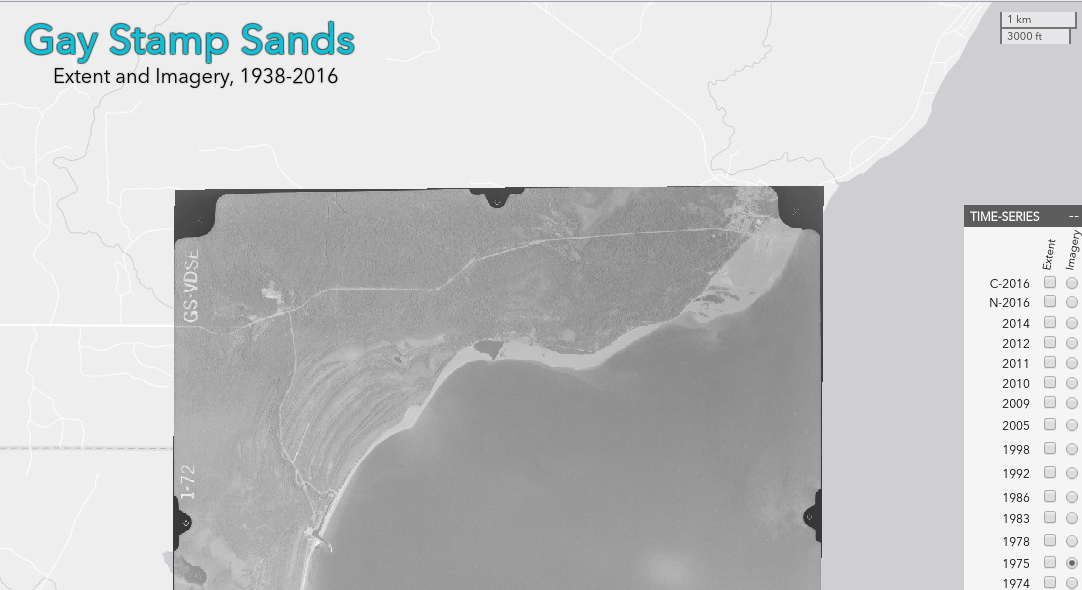
\includegraphics[width=1\textwidth]{../img/gay-sands.png}
	\caption{screenshot zobrazující webovou platformu Gay Stand
Sands a její uživatelské rozhraní}
	\label{fig:gay-sands}
\end{figure}

\newpage
\subsection{GeoServer}

\begin{figure}[h!]  \centering

\includegraphics[width=0.4\textwidth]{../img/geoserver-logo.png}
	\label{fig:geoserver-logo}
\end{figure} \bigskip

Stejně jako u MapServeru se jedná o serverový program s otevřeným
kódem. GeoServer je napsán v Jazyce Java a umožňuje, na základě
otevřených standardů poskytovaných organizací OGC, sdílet a upravovat
geografická data ze všech hlavních datových zdrojů.

GeoServer vznikl v roce 2001 v neziskovém technologickém inkubátoru
\textit{The Open Planning Project} ve městě New York. V té době bylo
hlavním cílem vytvoření sady nástrojů, který umožní větší vládní
průhlednost. Jako první nástroj vznikl právě GeoServer. Pomocí něj
mohli být občané lépe zapojeni do vládních záležitostí, především
územního plánování.

\begin{figure}[h!]  \centering
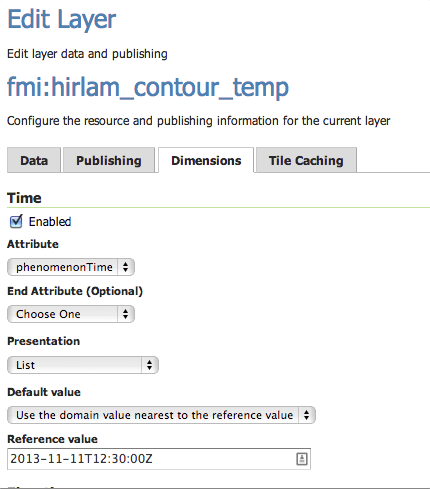
\includegraphics[width=0.6\textwidth]{../img/geoserver-layer-edit.png}
	\caption{záložka konfigurace časové vrstvy na GeoServeru
\cite{geoserver-layer-edit}}
	\label{fig:geoserver-layer-edit}
\end{figure}

\bigskip
\noindent

\textbf{Podpora časových dat}

Podpora časoprostorových dat na straně GeoServeru je dost podobná té v
MapServeru. GeoServer podporuje v operaci \textit{GetMap} atribut
\textit{TIME}. Pro jeho použití je nutné mít správně nastavenou
vrstvu, která časová data obsahuje.

Nejjednodušším způsobem nastavení vrstvy je využití webového rozhraní
pro GeoServer viz. obrázek 3. V záložce \textit{Dimensions} je veškeré
nutné nastavení. V případě nastavení časové vrstvy je potřeba nejprve
zaškrtnout políčko \textit{Time Enabled}. Další nastavení je
následující \cite{geoserver-layer-edit}:

\begin{itemize}
	\item \textit{Attribute} - zde je nutné vybrat atribut, který
obsahuje časovou složku. Na základě něj jsou zjištěny časové
hodnoty. Volba atributu je možná pouze pro vektorové vrstvy.
	\item \textit{End Attribute} - jedná se o nepovinné
pole. Pomocí \textit{End Attribute} je nastavena horní hranice
intervalu hodnot pro které je daný mapový prvek zobrazován.
	\item \textit{Presentation} - nastavení prezentace dat pro
\textit{GetCapabilities} operaci. Pokud jsou hodnoty diskrétní, tak je
možné nastavit možnost \textit{List}, \textit{interval and resolution}
pro hodnoty v intervalu s daným krokem, nebo \textit{continuous
interval} pro souvislý interval hodnot. Možnost \textit{List} je
vhodná například pro aplikace využívající animací, kdy jeden časový
okamžik odpovídá jednomu snímku animace.
	\item \textit{Default value} - jedná se o hodnotu, která
zastupuje data, která pro zvolený atribut neobsahují žádnou časovou
hodnotu. existuje několik možností jak \textit{Default value} zvolit:
	\begin{itemize}
		\item \textit{smallest domain value} - uloží nejnižší
hodnotu časového atributu
		\item \textit{biggest domain value} - uloží nejvyšší
hodnotu časového atributu
		\item \textit{nearest to the reference value} - uloží
hodnotu časového atributu, která je nejblíže dané referenční hodnotě
(\textit{Reference value})
		\item \textit{reference value} - uloží danou
referenční hodnotu tak jak je nehledě na to jestli je její použití
vhodné.
	\end{itemize}
	\item \textit{Reference value} - pole pro zvolení referenční
hodnoty sloužící při určení \textit{Default value}.
\end{itemize}

\bigskip
\noindent \textbf{Formáty časových dat a syntaxe}

\noindent Obecná syntaxe pro request s konkrétní hodnotou parametru
\textit{TIME} vypadá následovně:

\begin{verbatim} TIME=<timestring>
\end{verbatim}

Parametr \textit{TIME} je při \textit{GetMap} requestu vždy aplikován
na všechny aktuálně aktivní vrstvy definované parametrem
\textit{LAYERS}. Vrstvy bez časové složky tedy nejsou parametrem
\textit{TIME} nijak ovlivněny.

Pro zobrazení jednotlivých časových hodnot, intervalu a více hodnot je
syntaxe následující \cite{geoserver-time}:

\begin{itemize}
	\item TIME=2004-10-12 \textit{pro jednu konkrétní hodnotu
atributu.}
	\item TIME=2004-10-12,2004-10-13,2004-10-14 \textit{pro více
daných hodnot.}
	\item TIME=2004-10-12/2004-10-13 \textit{pro jeden konkrétní
interval hodnot.}
	\item TIME=2004-10-12/2004-10-13,2004-10-15/2004-10-16
\textit{pro více intervalů.}
\end{itemize}

Na první pohled je vidět, že rozdíl v syntaxi oproti MapServeru je
minimální. Mapserver však nabízí navíc možnost specifikace relativních
časových intervalů. Namísto přesné specifikace začátku a konce
intervalu je možné specifikovat začátek, nebo konec intervalu a přidat
dobu jeho trvání. Začátek či konec intervalu je zadán stejným
formátem, který je zobrazen výše. Pro hodnotu aktuálního času je možné
časovou hodnotu nahradit slovem \textit{PRESENT}.

Syntaxe pro specifikování relativních intervalů je
následující\cite{geoserver-time}:

\begin{itemize}
	\item TIME=2002-09-01T00:00:00.0Z/P1M \textit{pro interval
hodnot pokrývající celý měsíc září 2002. Pro celý den prvního září
2002 by bylo možné použít hodnotu} P1D.
	\item TIME=P1D/2010-12-25T00:00:00.0Z \textit{pro interval
hodnot pokrývající celý den 24. prosince 2010.}
	\item TIME=PT36H/PRESENT \textit{pro časový interval 36 hodin
v minulosti od aktuálního časového okamžiku.}
\end{itemize}

\bigskip
\noindent \textbf{Webové mapové platformy}

%nejsem si jist jestli je na GeoServeru \textbf{MetEye}
(http://www.bom.gov.au/australia/meteye) je webová mapová platforma
zobrazující meterologické observace a předpovědí pro celý australský
kontinent. Jedná se o interaktivní mapovou platformu vytvořenou
Australským úřadem pro metorologii (Australian Bureaou of Metorologi).

Webové rozhraní obsahuje panel s tématickými mapy, pomocí kterých se
dá mapový obsah modifikovat. Zde lze vybrat typ předpovědi jako
například vodní srážky, teplotu, sílu a směr větru atd. Mapové okno
mimo standartních mapových prvků jako jsou legenda a grafické měřítko
nabízí rovněž možnost zobrazení předpovědi počasí pro daný časový
okamžik. Toho je docíleno pomoci velice pěkně zpracované časové osy v
horní části mapového okna. Zde lze data rovněž data po časových
úsecích animovat.

Rastrové vrstvy jsou filtrovány na základě parametru
\textit{TIMESTAMP}, který je vždy shodný u všech dlaždic. Vzhledem k
tomu, že pro jednotlivé předpovědi se mění pouze rastrové vrstvy, je
možné je na webovém serveru cashovat a distribuovat ve formě dlaždic.

\begin{figure}[h!]  \centering
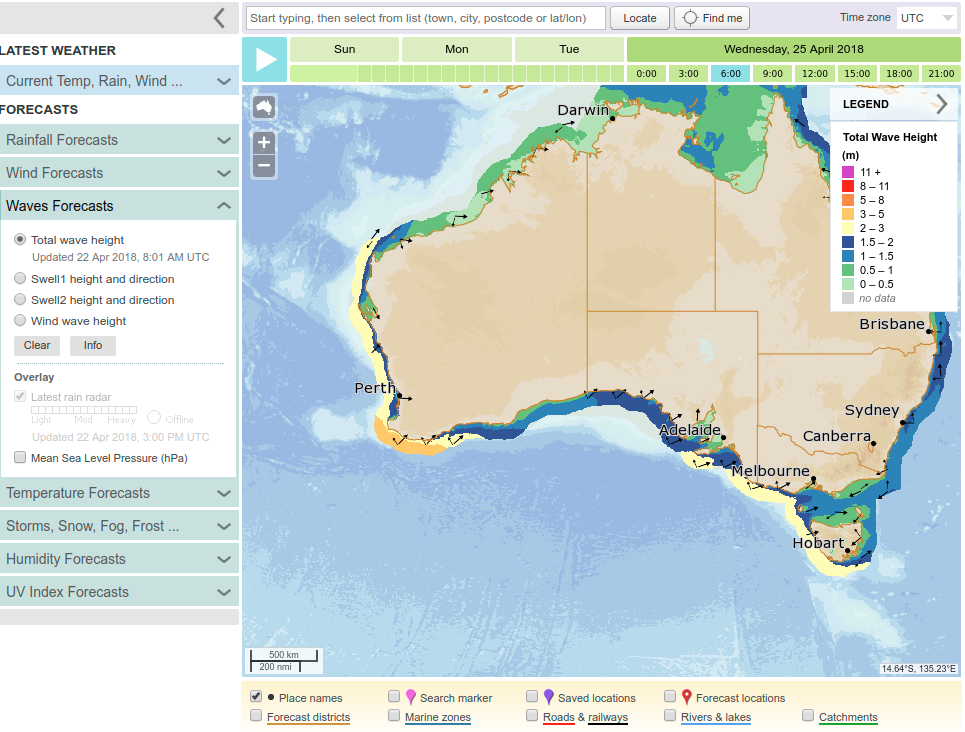
\includegraphics[width=0.67\textwidth]{../img/meteye.png}
	\caption{screenshot zobrazující webovou platformu MetEye}
	\label{fig:gay-sands}
\end{figure}

\textbf{Pennsylvania Cancer Atlas}
(https://www.geovista.psu.edu/grants/CDC/) je webová platforma
zobrazující výskyt rakoviny prostaty a tlustého střeva ve státě
Pensylvánie na severovýchodě USA. V tomto případě se jedná o webovou
mapovou aplikaci využívající software Adobe Flash Player, který se
spouští pomoci webového prohlížeče.

Uživatelské rozhraní nabízí tématickou mapu celého státu, která je
rozdělena na regiony. Ty jsou barevně zvýrazněny dle zastoupení
rakoviny v populaci. Pro každé období jsou dále vyhotoveny celostátní
statistiky, které jsou zobrazeny v grafech a tabulce okolo. Data jsou
sbírána pro období jednoho až dvou let a pomoci jednoduchého
roletového menu je možné jednotlivě je selektovat, nebo spustit
animaci. Zde pomocí panelu animace jde animaci spustit, kdy se
jednotlivá období střídají s předem daným časovým krokem. Ten dále
nabízí přeskočení na následující období a ukončení animování.

\begin{figure}[h!]  \centering
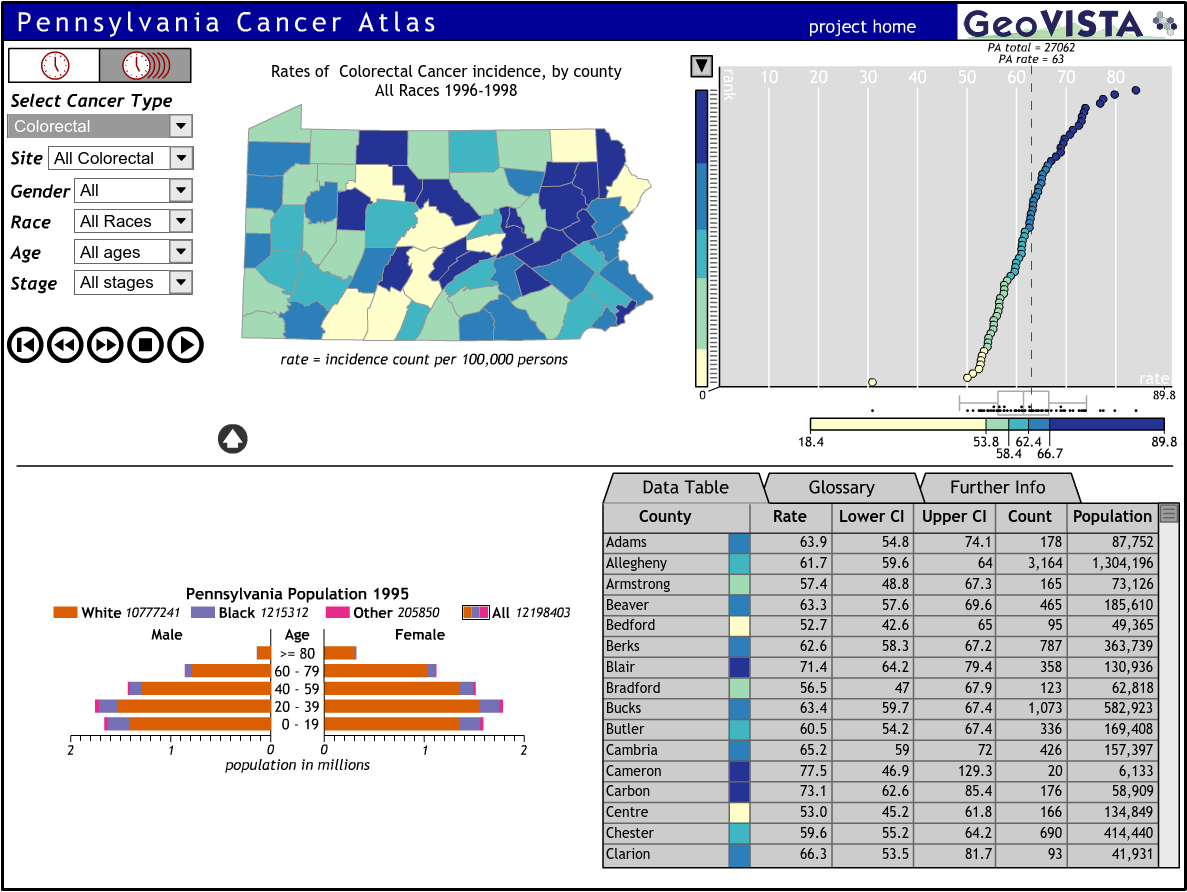
\includegraphics[width=0.8\textwidth]{../img/pennsylvania-cancer-atlas.png}
	\caption{screenshot zobrazující webovou platformu Pennsylvania
Cancer Atlas a její uživatelské rozhraní s možností animace dle
časového období statistik}
	\label{fig:gay-sands}
\end{figure}
 
\newpage
\subsection{ArcGIS}

\begin{figure}[h!]  \centering

\includegraphics[width=0.4\textwidth]{../img/arcgis-logo.jpg}
	\label{fig:arcgis-logo}
\end{figure} \bigskip

ArcGIS je platforma obsahující řadu aplikací které společně tvoří
geografický informační systém sloužící pro práci s prostorovými
daty. Nejedná se tedy o webový mapový server jako takový. ArcGIS je
soukromý systém vytvořený firmou Esri (Environmental Systems Research
Institute). Ta již v devedesátých letech pracovala na GIS
aplikacích. V roce 1999 byla vydána desktopová aplikace ArcMap 8.0
(později přejmenovaná na ArcGIS Desktop a poté pouze na ArcGIS), která
se od té doby stala nejpoužívanější komerčním softwarem na poli
geografických informačních systémů \cite{arcgis_history}.

Pod ArcGis mimo jiné patří aplikace pro webovou mapovou
publikaci. Jedná se o \textbf{ArcGIS server}, \textbf{ArcGIS Online} a
\textbf{Portal for ArcGIS}. Součástí posledního jmenovaného systému je
již zmíněný ArcGIS server, proto se mu v další části není potřeba dále
věnovat.

\newpage
\subsection{ArcGIS server}

Jedná o službu zahrnující mapování, geoprocessing, obrazové a síťové
analýzy, 3D data a možnost tvorby geografických prvků
\cite{arcgis-publishing-service}. Funkcionalita ArcGIS serveru se liší
dle balíčků, které na základě ceny omezují jeho možnosti.

\bigskip
\noindent \textbf{Podpora časových dat}
 
ArcGIS nabízí možnost pracování s vrstvy obsahující časová data. K
tomu je nutné jednotlivé vrstvy ještě před jejich publikací
nastavit. V desktopové aplikaci k tomu slouží dialogové okno, které je
možné nalézt v nastavení vrstev.

\begin{figure}[h!]  \centering
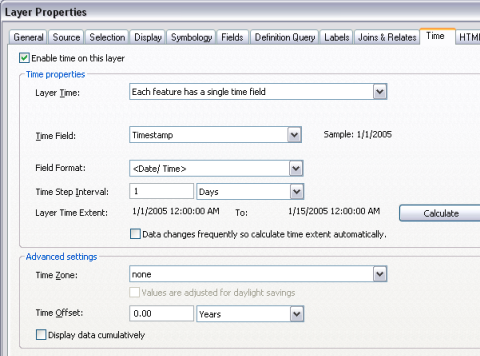
\includegraphics[width=0.8\textwidth]{../img/arcgis-layer-edit.png}
	\caption{dialogové okno nastavení časové vrstvy v desktopové
aplikaci ArcGIS}
	\label{fig:arcgis-time-settings}
\end{figure}

K možnosti publikace je nejprve zaškrtnout možnost \textit{Enable time
on this layer} tím bude vrstva jasně identifikována jako časová. Dále
je nutno specifikovat jakým způsobem jsou časové hodnoty v datech
uloženy. Ty mohou být jako atributové pole pro vektorová data, nebo
jako rastrový katalog pro rastrová data. Nutné je rovněž nastavení
kroku, který by měl co nejlépe korespondovat s krokem v jakém jsou
jednotlivá data pořízena. Následující pole slouží k nastavení:

\begin{itemize}
	\item \textit{Time Properties} - v roletovém menu
\textit{Layer Time} je možnost zvolit jestli data jsou pouze v jednom
atributovém poli, nebo ve dvou. V tom případě jeden obsahuje začátek a
druhý konec časového intervalu. Konkrétní názvy atributů je dále nutné
zvolit z nabídky atributů pro příslušnou vrstvu. Pokud formát
atributu, kde jsou časová data uložena nepodporuje časová data
např. řetězec, nebo číselná hodnota, je nutné daný formát dále
specifikovat. Poté je možné pomocí tlačítka \textit{Calculate}
vypočítat časový rozsah. Tato hodnota je posléze použita k
inicializaci časového posuvníku a rovněž k validaci časových dat. Po
výpočtu je vypsán doporučený krok určený pro časový posuvník. Velikost
kroku lze případně změnit.
	
	\item \textit{Time Properties} - část s rozšířeným nastavením
není povinné nijak modifikovat. Obsahuje možnost specifikování časové
zóny pro použitá časová data. Takové nastavení je vhodné především pro
publikací více časových vrstev obsahující data z jiných časových
pásem. Pokud jsou jejich pásma specifikována lze tato data snadno
kombinovat dohromady. Stejného výsledku lze také dosáhnout pomoci
nastavení časového posunu níže. V případě že jsou některá časová data
pořízena v zemích používající změnu času na čas letní \textit{daylight
saving time}, nabízí ArcGIS tuto skutečnost u dat
specifikovat. Poslední možnost, kterou tato sekce nabízí je
\textit{Display data cumulatively} tedy kumulativní zobrazení dat. V
tom případě jsou zobrazena veškerá data mající počáteční časovou
hodnotu stejnou, nebo menší, než aktuálně zvolenou. Pokud taková data
mají nastavený konec časového intervalu je tato hodnota ignorována.
\end{itemize}

Takto nastavené vrstvy lze publikovat na ArcGIS server a pomocí
webových mapových servisů vytvářet požadované mapové obrazy. K jejich
finálnímu použití je však nutné mapový projekt publikovat na
server. Proces publikace již žádné dodatečné nastavení pro vrstvy
obsahující časová data neobsahuje, proto se mu tato kapitola věnovat
nebude. V kostce s jedná o jednoduché nastavení servisu pomocí
dialogového okna s možností náhledu projektu.

\bigskip
\noindent \textbf{Formáty časových dat a syntaxe}

Jak již bylo řečeno časové hodnoty jsou podporovány ve třech datových
typech. Datový typ podporující datum, textový řetězec a číselná
hodnota. Pro nižší výpočetní náročnost je doporučeno datové typy
podporující datum maximálně využívat. V případě textových řetězců je
podporováno 13 formátů a v případě číselných hodnot se jedná o 4
formáty \cite{arcgiq-data-types}.  %moznost pridat formaty

\subsection{ArcGIS Online}

ArcGIS online nabízí uživatelům publikování projektu přímo do cloudové
služby spravované společností ArcGIS. Jedná se o velice jednoduchý
způsob publikace, kdy si není potřeba instalovat žádný software, nutné
je pouze vytvořit účet. Nabízené jsou dva hlavní typy
publikace. Jejich použití závisí na konkrétním použití aplikace. Pro
větší projekty je poté vhodná také jejich kombinace
\cite{arcgis-publishing-service}:
\begin{itemize}
	\item \textit{Feature services} - slouží především pro
publikaci atributů, mapových symbolů a dalších informací. Tyto mapové
objekty bývají často zobrazeny spolu s podkladovou mapou.
	\item \textit{Tiled map services} - jak již název napovídá,
jedná se o sadu předem generovaných mapových snímků, které jsou
serverem distribuovány ve formě mapových dlaždic. Ty mohou být pro
zvýšení výkonu aplikace drženy v mezipaměti serveru, odkud jsou přímo
dostupně přes jejich URL.
\end{itemize}

\bigskip
\noindent \textbf{Podpora časových dat} Stejně jako předchozí produkt
\textit{ArcGIS server}, tak \textit{ArcGIS online} nabízí taktéž
podporu pro práci s časoprostorovými daty. Nastavení se však liší a
vzhledem k již definovanému uživatelskému rozhraní jsou možnosti
použití rovněž omezeny na předem dané nástroje.

K tomu, aby mohla být daná vrstva označena jako časová, musí splňovat
dvě základní podmínky. Vrstva musí být typu \textit{feature layer},
\textit{map image layer}, \textit{imagery layer}, to jsou typy vrstev
podporující časové animace. Druhou podmínkou je označení konkrétní
vrstvy jako \textit{time enabled} tedy jako vrstvu podporující časová
data. Ověření podpory časových dat lze provést v \textit{map viewer} v
detailu vrstvy. Pro označení vrstvy jako časové je nutné provést kroky
popsané v podkapitole 2.4 (sekce Podpora časových dat). Pokud vrstva
splňuje obě podmínky a je označena jako viditelná zobrazí se ve spodní
části mapového prohlížeče nástroj pro správu časové vrstvy.

\begin{figure}[h!]  \centering

\includegraphics[width=0.8\textwidth]{../img/arcgis-online-time-slider.png}
	\caption{nástroj pro správu časových vrstev}
	\label{fig:arcgis-time-settings}
\end{figure}

%vice detalneji? moznost obrazku a popisu detailniho nastaveni
casoveho nastroje Nástroj obsahuje časovou osu s posuvníky, tlačítka
pro vytvoření animace a tlačítko časového nastavení \textit{time
settings}. Po rozkliknutí tlačítka časového nastavení se zobrazí
dialogové okno, které umožňuje konfiguraci časové osy. Nastavení
dovoluje pro účely animace vrstvy změnit dobu trvání jednoho
snímku. Dále je možné omezit časovou osu jen na daný časový
interval. Implicitně je interval definován jako minimální a maximální
časová hodnota sjednocení intervalů časových hodnot pro všechny
vrstvy. V případě že není nastaveno kumulativní zobrazení dat, je
možné nastavit velikost intervalu pro který se v daný okamžik časová
data zobrazují.

Nastavení v detailu vrstvy rovněž umožňuje časový nástroj pro vrstvu
podporující časová data deaktivovat.

\newpage
\subsection{QGIS server}

Jedná se o mapový webový server s otevřenými daty implementující
pokročilé mapové prvky pro tvorbu tématických map. Zdrojový kód je
napsaný v programovacím jazyce C++, jsou v něm však podporované
zásuvné moduly psané jazykem Python, které umožňují rychlé a efektivní
vývoj nových komponent serveru a jeho rozšíření. V QGIS serveru jsou
implementovány standarty definované organizací OGC WMS 1.3, WFS 1.0.0
a WCS 1. Jeho vývoj byl podporován projekty Evropské unie Orchestra a
Sany a dále městem Uster ve Švýcarsku \cite{qgis-server}.

Výhoda použití QGIS serveru spočívá v použití stejné logiky jako u
desktopového QGIS. Pro vytváření map jsou použity stejné vizualizační
knihovny, které zároveň aplikují kartografická pravidla. To ve
výsledku znamená, že mapy publikované na webové publikační platformě s
použitím QGIS serveru budou vypadat stejně jako v desktopovém QGIS.

\bigskip
\noindent \textbf{Podpora časových dat}

QGIS server oproti ostatním zmíněným systémům nijak podporu pro data s
časovou složkou nepodporuje. Filtrace dat na základě parametru
\textit{TIME} tedy není možná.

Pro výše zmíněnou výhodu Qisquick platforma QGIS server používá. V
Druhé části práce bude popsáno jakým způsobem je možnost práce s
časoprostorovými daty s použitím QGIS serveru implementována.

\newpage
\subsection{Souhrn} V předešlých kapitolách byly popsány jednotlivé
principy a postupy práce s časoprostorovými daty pro rozdílné mapové
servery a mapové publikační platformy. Již na první pohled je zřejmé
že i přes dílčí rozdíly jsou ve všech aplikacích použita podobná
nastavení a pravidla.

\bigskip
\noindent \textbf{MapServer}
\begin{itemize}
	\item software s otevřeným kódem užívající OGC standarty,
volně dostupný pro každého uživatele
	\item široká podpora časových formátů
	\item validace vstupních časových dat na základě definované
masky
	\item možnost filtrace konkrétních hodnot i intervalů hodnot
	\item možnost definice hodnoty prvku v případě neexistující
hodnoty
\end{itemize}

\textbf{GeoServer}
\begin{itemize}
	\item software s otevřeným kódem užívající OGC standarty,
volně dostupný pro každého uživatele
	\item možnost konfigurace časových vrstev v uživatelském
rozhraní
	\item mapové prvky můžou obsahovat časovou hodnotu, nebo
interval hodnot ve kterém jsou zobrazovány
	\item možnost filtrace konkrétních hodnot i intervalů hodnot
	\item velká nabídka způsobů definice hodnoty prvku v případě
neexistující hodnoty
\end{itemize}

\textbf{ArcGIS server}
\begin{itemize}
	\item nutnost zakoupení licence pro daný software
	\item široká podpora časových a datových formátů
	\item konfigurace časových vrstev je možná v desktopové
aplikaci
	\item obrovská nabídka možností konfigurace časových vrstev
	\item mapové prvky můžou obsahovat časovou hodnotu, nebo
interval hodnot ve kterém jsou zobrazovány
	\item možnost filtrace konkrétních hodnot i intervalů hodnot
\end{itemize}

\textbf{ArcGIS online}
\begin{itemize}
	\item nutnost zakoupení licence pro daný software
	\item práce v cloudu, není nutná instalace software
	\item široká podpora časových a datových formátů
	\item konfigurace časových vrstev je možná v desktopové
aplikaci
	\item obrovská nabídka možností konfigurace časových vrstev
	\item mapové prvky můžou obsahovat časovou hodnotu, nebo
interval hodnot ve kterém jsou zobrazovány
	\item možnost filtrace konkrétních hodnot i intervalů hodnot
	\item přímá integrace nástrojů pro práci s časoprostorovými
daty
\end{itemize}

 
%https://gis.stackexchange.com/questions/12493/list-of-map-service-software?utm_medium=organic&utm_source=google_rich_qa&utm_campaign=google_rich_qa

% qgis server % qgis clound
%https://gis.stackexchange.com/questions/34667/does-qgis-have-wms-t-wms-with-time-support?rq=1
%https://docs.qgis.org/2.18/en/docs/user_manual/working_with_ogc/ogc_server_support.html

% arcgis server
%https://enterprise.arcgis.com/en/server/latest/publish-services/linux/serving-time-aware-layers.htm
%https://developers.arcgis.com/javascript/3/jshelp/inside_temporal.html

%notes %http://tiles.metgis.com/tiles-demo/

%arcgis online
 
